
%% HUH Colloquium Presentation
%% Tom Eichlersmith

\documentclass{beamer}

\mode<presentation> {
	\usetheme{Goettingen}
	\setbeamertemplate{navigation symbols}{}
	\setbeamertemplate{footline}[page number]
}

\usepackage{graphicx} % Allows including images
\usepackage{booktabs} % Allows the use of \toprule, \midrule and \bottomrule in tables
\usepackage{subfigure} % For images next to each other
\usepackage{tikz} % Diagrams from dia

%-----------------------------------------------
%%	TITLE PAGE
%-----------------------------------------------

\title[Random Walks]{Random Walks on Simple Two-Dimensional Manifolds} % The short title appears at the bottom of every slide, the full title is only on the title page

\author{Tom Eichlersmith}
\institute[Hamline U]
{
Hamline University \\
\medskip
\texttt{teichlersmith01@hamline.edu}
}
\date{April 19, 2018}

\begin{document}

\begin{frame}
	\titlepage % Print the title page as the first slide
\end{frame}

%------------------------------------------------
%%	PRESENTATION SLIDES
%------------------------------------------------

\section{Introduction} 

\begin{frame}

	\frametitle{Introduction}
	
	\begin{itemize}
		\item Random
		\item Walk
		\item Simple
		\item Two-Dimensional
		\item Manifolds
	\end{itemize}

\end{frame}

%------------------------------------------------
\section{Background}

\begin{frame}
	
	\frametitle{}
	
\end{frame}

\begin{frame}

	\frametitle{Regular Surfaces}
	
	\begin{figure}
		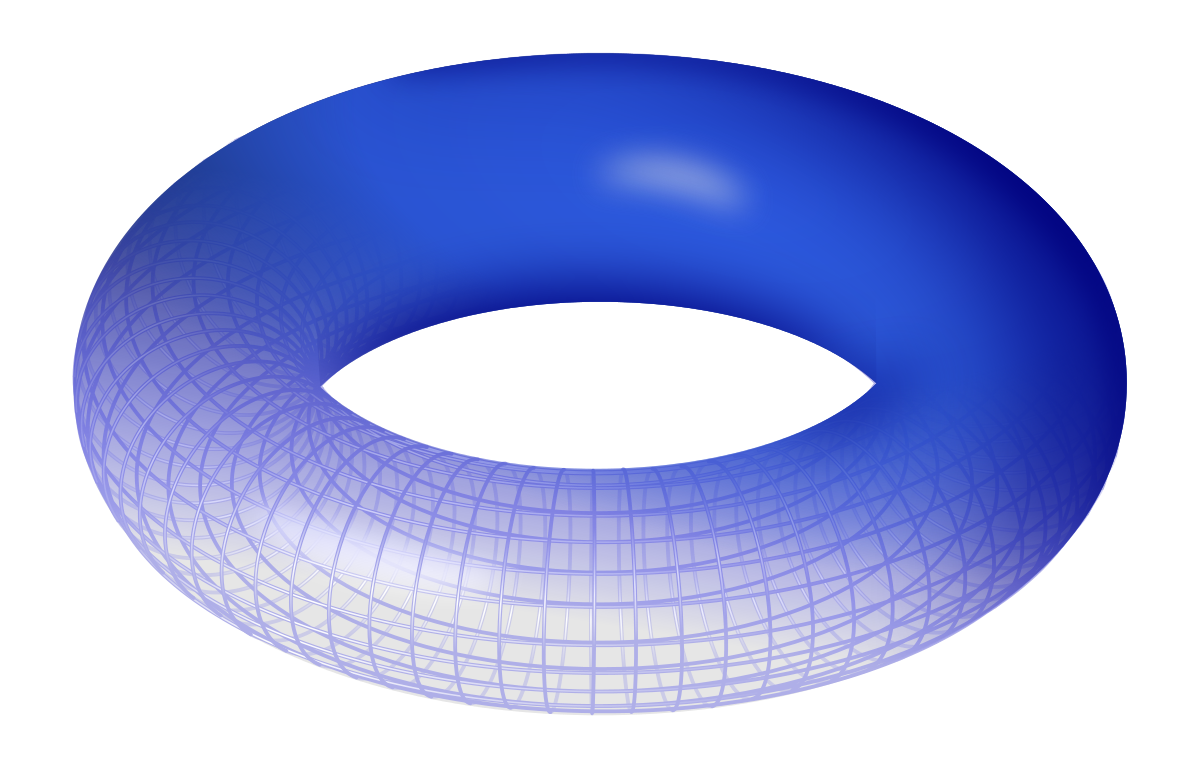
\includegraphics[width=\textwidth]{images/Torus.png}
		\caption{By Leonid\_2 - Own work, CC BY-SA 3.0, \texttt{https://commons.wikimedia.org/w/index.php?curid=8643414}}
	\end{figure}
	
\end{frame}

%---------------------------------------------------------------

\begin{frame}
	
	\frametitle{Geodesic Equations}
	
	\begin{enumerate}
		\item Extend definition of line to other surfaces
		\item Assume a path is a geodesic contained in a coordinate patch
		\item Derive geodesic equations for coordinate functions of path
	\end{enumerate}

\end{frame}

%---------------------------------------------------------------

\begin{frame}
	
	\frametitle{Geodesic Equations}
	
	\begin{align*}
		u'' + \frac{\mu_{uu} \cdot \mu_u}{\mu_u \cdot \mu_u} (u')^2 + \frac{\mu_{vv} \cdot \mu_u}{\mu_u \cdot \mu_u} (v')^2 + 2\frac{\mu_{uv} \cdot \mu_u}{\mu_u \cdot \mu_u} u'v' & = 0 \\
		v'' + \frac{\mu_{uu} \cdot \mu_v}{\mu_v \cdot \mu_v} (u')^2 + \frac{\mu_{vv} \cdot \mu_v}{\mu_v \cdot \mu_v} (v')^2 + 2\frac{\mu_{uv} \cdot \mu_v}{\mu_v \cdot \mu_v} u'v' & = 0 \\
	\end{align*}
	
	
\end{frame}

%---------------------------------------------------------------

\begin{frame}
	
	\frametitle{Christoffel Symbols}
	
	\begin{equation*} 
		\Gamma^i_{jk} = \frac{\mu_{jk}\cdot\mu_i}{\mu_i\cdot\mu_i} \quad\text{where } i,j,k \in \{u,v\}
	\end{equation*}
	
	$$\Big\Downarrow \text{abuse of symbols}$$
	
	\begin{equation*}
		\frac{d^2x^i}{dt^2} + \sum_{j,k \in \{1,2\}} \Gamma^i_{jk}\frac{dx^j}{dt}\frac{dx^k}{dt} = 0
	\end{equation*}
	
\end{frame}

%------------------------------------------------
\section{Method}

\begin{frame}

	\frametitle{Stepping Method}
	
	Runge-Kutta 4th Order Method (RK4)
	\begin{equation*}
		\frac{dy}{dt} = F(y) \quad y_0 = y(0)
	\end{equation*}
	Numerically solve up to $t=h$ with $N$ iterations.
	\begin{align*}
		& \delta \gets h/N \\
		& y \gets y_0 \\
		& \textit{loop } N \textit{ times:} \\
		& \quad\quad k_1 \gets F(y) \\
		& \quad\quad k_2 \gets F\left(y+(\delta/2)k_1\right) \\
		& \quad\quad k_3 \gets F\left(y+(\delta/2)k_2\right) \\
		& \quad\quad k_4 \gets F\left(y + \delta k_3\right) \\
		& \quad\quad y \gets y+(\delta/6)(k_1+2k_2+2k_3+k_4)
	\end{align*}

\end{frame}

%---------------------------------------------------------------

\begin{frame}
	
	\frametitle{Stepping Method}
	
	Define
	\begin{equation*}
		p = \frac{du}{dt} \quad\text{and}\quad q = \frac{dv}{dt}
	\end{equation*}
	Then the geodesic equations become
	\begin{align*}
		\frac{du}{dt} & = p \\
		\frac{dv}{dt} & = q \\
		\frac{dp}{dt} & = -\Gamma^u_{uu}p^2-2\Gamma^u_{uv}pq-\Gamma^u_{vv}q^2 \\
		\frac{dq}{dt} & = -\Gamma^v_{uu}p^2-2\Gamma^v_{uv}pq-\Gamma^v_{vv}q^2 \\
	\end{align*}
	
\end{frame}

%---------------------------------------------------------------

\begin{frame}
	
	\frametitle{Coordinate Wrapping}
	
	\begin{figure}
		% Graphic for TeX using PGF
% Title: /home/tom/CodeProjects/MathDHP_201718/RandomManifoldWalks/Presentation/images/TorusWrap.dia
% Creator: Dia v0.97.3
% CreationDate: Sun Apr  8 19:46:43 2018
% For: tom
% \usepackage{tikz}
% The following commands are not supported in PSTricks at present
% We define them conditionally, so when they are implemented,
% this pgf file will use them.
\ifx\du\undefined
  \newlength{\du}
\fi
\setlength{\du}{15\unitlength}
\begin{tikzpicture}
\pgftransformxscale{1.000000}
\pgftransformyscale{-1.000000}
\definecolor{dialinecolor}{rgb}{0.000000, 0.000000, 0.000000}
\pgfsetstrokecolor{dialinecolor}
\definecolor{dialinecolor}{rgb}{1.000000, 1.000000, 1.000000}
\pgfsetfillcolor{dialinecolor}
\pgfsetlinewidth{0.100000\du}
\pgfsetdash{}{0pt}
\pgfsetdash{}{0pt}
\pgfsetbuttcap
\pgfsetmiterjoin
\pgfsetlinewidth{0.100000\du}
\pgfsetbuttcap
\pgfsetmiterjoin
\pgfsetdash{}{0pt}
\definecolor{dialinecolor}{rgb}{0.000000, 0.000000, 0.000000}
\pgfsetstrokecolor{dialinecolor}
\draw (5.000000\du,10.000000\du)--(5.000000\du,21.000000\du)--(15.645161\du,21.000000\du)--(15.645161\du,10.000000\du)--cycle;
\pgfsetbuttcap
\pgfsetmiterjoin
\pgfsetdash{}{0pt}
\definecolor{dialinecolor}{rgb}{0.000000, 0.000000, 0.000000}
\pgfsetstrokecolor{dialinecolor}
\draw (5.000000\du,10.000000\du)--(5.000000\du,21.000000\du)--(15.645161\du,21.000000\du)--(15.645161\du,10.000000\du)--cycle;
\pgfsetlinewidth{0.100000\du}
\pgfsetdash{}{0pt}
\pgfsetdash{}{0pt}
\pgfsetbuttcap
{
\definecolor{dialinecolor}{rgb}{0.000000, 0.000000, 0.000000}
\pgfsetfillcolor{dialinecolor}
% was here!!!
}
\definecolor{dialinecolor}{rgb}{0.000000, 0.000000, 0.000000}
\pgfsetstrokecolor{dialinecolor}
\draw (4.000000\du,19.000000\du)--(5.513197\du,19.000000\du);
\pgfsetlinewidth{0.100000\du}
\pgfsetdash{}{0pt}
\pgfsetmiterjoin
\definecolor{dialinecolor}{rgb}{0.000000, 0.000000, 0.000000}
\pgfsetstrokecolor{dialinecolor}
\draw (4.500000\du,19.000000\du)--(4.000000\du,18.750000\du);
\definecolor{dialinecolor}{rgb}{0.000000, 0.000000, 0.000000}
\pgfsetstrokecolor{dialinecolor}
\draw (4.500000\du,19.000000\du)--(4.000000\du,19.250000\du);
\pgfsetdash{}{0pt}
\pgfsetmiterjoin
\pgfsetbuttcap
\definecolor{dialinecolor}{rgb}{0.000000, 0.000000, 0.000000}
\pgfsetstrokecolor{dialinecolor}
\draw (5.888197\du,19.000000\du)--(5.388197\du,19.250000\du)--(5.513197\du,19.000000\du)--(5.388197\du,18.750000\du)--cycle;
\pgfsetlinewidth{0.100000\du}
\pgfsetdash{}{0pt}
\pgfsetdash{}{0pt}
\pgfsetbuttcap
{
\definecolor{dialinecolor}{rgb}{0.000000, 0.000000, 0.000000}
\pgfsetfillcolor{dialinecolor}
% was here!!!
}
\definecolor{dialinecolor}{rgb}{0.000000, 0.000000, 0.000000}
\pgfsetstrokecolor{dialinecolor}
\draw (14.400000\du,19.000000\du)--(15.913197\du,19.000000\du);
\pgfsetlinewidth{0.100000\du}
\pgfsetdash{}{0pt}
\pgfsetmiterjoin
\definecolor{dialinecolor}{rgb}{0.000000, 0.000000, 0.000000}
\pgfsetstrokecolor{dialinecolor}
\draw (14.900000\du,19.000000\du)--(14.400000\du,18.750000\du);
\definecolor{dialinecolor}{rgb}{0.000000, 0.000000, 0.000000}
\pgfsetstrokecolor{dialinecolor}
\draw (14.900000\du,19.000000\du)--(14.400000\du,19.250000\du);
\pgfsetdash{}{0pt}
\pgfsetmiterjoin
\pgfsetbuttcap
\definecolor{dialinecolor}{rgb}{0.000000, 0.000000, 0.000000}
\pgfsetstrokecolor{dialinecolor}
\draw (16.288197\du,19.000000\du)--(15.788197\du,19.250000\du)--(15.913197\du,19.000000\du)--(15.788197\du,18.750000\du)--cycle;
\pgfsetlinewidth{0.100000\du}
\pgfsetdash{}{0pt}
\pgfsetdash{}{0pt}
\pgfsetbuttcap
{
\definecolor{dialinecolor}{rgb}{0.000000, 0.000000, 0.000000}
\pgfsetfillcolor{dialinecolor}
% was here!!!
}
\definecolor{dialinecolor}{rgb}{0.000000, 0.000000, 0.000000}
\pgfsetstrokecolor{dialinecolor}
\draw (16.400000\du,12.000000\du)--(14.886803\du,12.000000\du);
\pgfsetlinewidth{0.100000\du}
\pgfsetdash{}{0pt}
\pgfsetmiterjoin
\definecolor{dialinecolor}{rgb}{0.000000, 0.000000, 0.000000}
\pgfsetstrokecolor{dialinecolor}
\draw (15.900000\du,12.000000\du)--(16.400000\du,12.250000\du);
\definecolor{dialinecolor}{rgb}{0.000000, 0.000000, 0.000000}
\pgfsetstrokecolor{dialinecolor}
\draw (15.900000\du,12.000000\du)--(16.400000\du,11.750000\du);
\pgfsetdash{}{0pt}
\pgfsetmiterjoin
\pgfsetbuttcap
\definecolor{dialinecolor}{rgb}{0.000000, 0.000000, 0.000000}
\pgfsetstrokecolor{dialinecolor}
\draw (14.511803\du,12.000000\du)--(15.011803\du,11.750000\du)--(14.886803\du,12.000000\du)--(15.011803\du,12.250000\du)--cycle;
\pgfsetlinewidth{0.100000\du}
\pgfsetdash{}{0pt}
\pgfsetdash{}{0pt}
\pgfsetbuttcap
{
\definecolor{dialinecolor}{rgb}{0.000000, 0.000000, 0.000000}
\pgfsetfillcolor{dialinecolor}
% was here!!!
}
\definecolor{dialinecolor}{rgb}{0.000000, 0.000000, 0.000000}
\pgfsetstrokecolor{dialinecolor}
\draw (6.000000\du,12.000000\du)--(4.486803\du,12.000000\du);
\pgfsetlinewidth{0.100000\du}
\pgfsetdash{}{0pt}
\pgfsetmiterjoin
\definecolor{dialinecolor}{rgb}{0.000000, 0.000000, 0.000000}
\pgfsetstrokecolor{dialinecolor}
\draw (5.500000\du,12.000000\du)--(6.000000\du,12.250000\du);
\definecolor{dialinecolor}{rgb}{0.000000, 0.000000, 0.000000}
\pgfsetstrokecolor{dialinecolor}
\draw (5.500000\du,12.000000\du)--(6.000000\du,11.750000\du);
\pgfsetdash{}{0pt}
\pgfsetmiterjoin
\pgfsetbuttcap
\definecolor{dialinecolor}{rgb}{0.000000, 0.000000, 0.000000}
\pgfsetstrokecolor{dialinecolor}
\draw (4.111803\du,12.000000\du)--(4.611803\du,11.750000\du)--(4.486803\du,12.000000\du)--(4.611803\du,12.250000\du)--cycle;
\pgfsetlinewidth{0.100000\du}
\pgfsetdash{}{0pt}
\pgfsetdash{}{0pt}
\pgfsetbuttcap
{
\definecolor{dialinecolor}{rgb}{0.000000, 0.000000, 0.000000}
\pgfsetfillcolor{dialinecolor}
% was here!!!
}
\definecolor{dialinecolor}{rgb}{0.000000, 0.000000, 0.000000}
\pgfsetstrokecolor{dialinecolor}
\draw (7.000000\du,20.000000\du)--(7.000000\du,21.513197\du);
\pgfsetlinewidth{0.100000\du}
\pgfsetdash{}{0pt}
\pgfsetmiterjoin
\definecolor{dialinecolor}{rgb}{0.000000, 0.000000, 0.000000}
\pgfsetstrokecolor{dialinecolor}
\draw (7.000000\du,20.500000\du)--(7.250000\du,20.000000\du);
\definecolor{dialinecolor}{rgb}{0.000000, 0.000000, 0.000000}
\pgfsetstrokecolor{dialinecolor}
\draw (7.000000\du,20.500000\du)--(6.750000\du,20.000000\du);
\pgfsetdash{}{0pt}
\pgfsetmiterjoin
\pgfsetbuttcap
\definecolor{dialinecolor}{rgb}{0.000000, 0.000000, 0.000000}
\pgfsetstrokecolor{dialinecolor}
\draw (7.000000\du,21.888197\du)--(6.750000\du,21.388197\du)--(7.000000\du,21.513197\du)--(7.250000\du,21.388197\du)--cycle;
\pgfsetlinewidth{0.100000\du}
\pgfsetdash{}{0pt}
\pgfsetdash{}{0pt}
\pgfsetbuttcap
{
\definecolor{dialinecolor}{rgb}{0.000000, 0.000000, 0.000000}
\pgfsetfillcolor{dialinecolor}
% was here!!!
}
\definecolor{dialinecolor}{rgb}{0.000000, 0.000000, 0.000000}
\pgfsetstrokecolor{dialinecolor}
\draw (7.000000\du,9.000000\du)--(7.000000\du,10.513197\du);
\pgfsetlinewidth{0.100000\du}
\pgfsetdash{}{0pt}
\pgfsetmiterjoin
\definecolor{dialinecolor}{rgb}{0.000000, 0.000000, 0.000000}
\pgfsetstrokecolor{dialinecolor}
\draw (7.000000\du,9.500000\du)--(7.250000\du,9.000000\du);
\definecolor{dialinecolor}{rgb}{0.000000, 0.000000, 0.000000}
\pgfsetstrokecolor{dialinecolor}
\draw (7.000000\du,9.500000\du)--(6.750000\du,9.000000\du);
\pgfsetdash{}{0pt}
\pgfsetmiterjoin
\pgfsetbuttcap
\definecolor{dialinecolor}{rgb}{0.000000, 0.000000, 0.000000}
\pgfsetstrokecolor{dialinecolor}
\draw (7.000000\du,10.888197\du)--(6.750000\du,10.388197\du)--(7.000000\du,10.513197\du)--(7.250000\du,10.388197\du)--cycle;
\pgfsetlinewidth{0.100000\du}
\pgfsetdash{}{0pt}
\pgfsetdash{}{0pt}
\pgfsetbuttcap
{
\definecolor{dialinecolor}{rgb}{0.000000, 0.000000, 0.000000}
\pgfsetfillcolor{dialinecolor}
% was here!!!
}
\definecolor{dialinecolor}{rgb}{0.000000, 0.000000, 0.000000}
\pgfsetstrokecolor{dialinecolor}
\draw (13.000000\du,22.000000\du)--(13.000000\du,20.486803\du);
\pgfsetlinewidth{0.100000\du}
\pgfsetdash{}{0pt}
\pgfsetmiterjoin
\definecolor{dialinecolor}{rgb}{0.000000, 0.000000, 0.000000}
\pgfsetstrokecolor{dialinecolor}
\draw (13.000000\du,21.500000\du)--(12.750000\du,22.000000\du);
\definecolor{dialinecolor}{rgb}{0.000000, 0.000000, 0.000000}
\pgfsetstrokecolor{dialinecolor}
\draw (13.000000\du,21.500000\du)--(13.250000\du,22.000000\du);
\pgfsetdash{}{0pt}
\pgfsetmiterjoin
\pgfsetbuttcap
\definecolor{dialinecolor}{rgb}{0.000000, 0.000000, 0.000000}
\pgfsetstrokecolor{dialinecolor}
\draw (13.000000\du,20.111803\du)--(13.250000\du,20.611803\du)--(13.000000\du,20.486803\du)--(12.750000\du,20.611803\du)--cycle;
\pgfsetlinewidth{0.100000\du}
\pgfsetdash{}{0pt}
\pgfsetdash{}{0pt}
\pgfsetbuttcap
{
\definecolor{dialinecolor}{rgb}{0.000000, 0.000000, 0.000000}
\pgfsetfillcolor{dialinecolor}
% was here!!!
}
\definecolor{dialinecolor}{rgb}{0.000000, 0.000000, 0.000000}
\pgfsetstrokecolor{dialinecolor}
\draw (13.000000\du,11.000000\du)--(13.000000\du,9.486803\du);
\pgfsetlinewidth{0.100000\du}
\pgfsetdash{}{0pt}
\pgfsetmiterjoin
\definecolor{dialinecolor}{rgb}{0.000000, 0.000000, 0.000000}
\pgfsetstrokecolor{dialinecolor}
\draw (13.000000\du,10.500000\du)--(12.750000\du,11.000000\du);
\definecolor{dialinecolor}{rgb}{0.000000, 0.000000, 0.000000}
\pgfsetstrokecolor{dialinecolor}
\draw (13.000000\du,10.500000\du)--(13.250000\du,11.000000\du);
\pgfsetdash{}{0pt}
\pgfsetmiterjoin
\pgfsetbuttcap
\definecolor{dialinecolor}{rgb}{0.000000, 0.000000, 0.000000}
\pgfsetstrokecolor{dialinecolor}
\draw (13.000000\du,9.111803\du)--(13.250000\du,9.611803\du)--(13.000000\du,9.486803\du)--(12.750000\du,9.611803\du)--cycle;
\pgfsetlinewidth{0.100000\du}
\pgfsetdash{}{0pt}
\pgfsetdash{}{0pt}
\pgfsetbuttcap
{
\definecolor{dialinecolor}{rgb}{0.000000, 0.000000, 1.000000}
\pgfsetfillcolor{dialinecolor}
% was here!!!
\definecolor{dialinecolor}{rgb}{0.000000, 0.000000, 1.000000}
\pgfsetstrokecolor{dialinecolor}
\draw (10.000000\du,15.000000\du)--(11.000000\du,15.000000\du);
}
\definecolor{dialinecolor}{rgb}{0.000000, 0.000000, 1.000000}
\pgfsetstrokecolor{dialinecolor}
\draw (10.000000\du,15.000000\du)--(10.750000\du,15.000000\du);
\pgfsetlinewidth{0.100000\du}
\pgfsetdash{}{0pt}
\pgfsetmiterjoin
\pgfsetbuttcap
\definecolor{dialinecolor}{rgb}{0.000000, 0.000000, 1.000000}
\pgfsetfillcolor{dialinecolor}
\pgfpathmoveto{\pgfpoint{11.000000\du}{15.000000\du}}
\pgfpathcurveto{\pgfpoint{11.000000\du}{15.075000\du}}{\pgfpoint{10.925000\du}{15.150000\du}}{\pgfpoint{10.850000\du}{15.150000\du}}
\pgfpathcurveto{\pgfpoint{10.775000\du}{15.150000\du}}{\pgfpoint{10.700000\du}{15.075000\du}}{\pgfpoint{10.700000\du}{15.000000\du}}
\pgfpathcurveto{\pgfpoint{10.700000\du}{14.925000\du}}{\pgfpoint{10.775000\du}{14.850000\du}}{\pgfpoint{10.850000\du}{14.850000\du}}
\pgfpathcurveto{\pgfpoint{10.925000\du}{14.850000\du}}{\pgfpoint{11.000000\du}{14.925000\du}}{\pgfpoint{11.000000\du}{15.000000\du}}
\pgfusepath{fill}
\definecolor{dialinecolor}{rgb}{0.000000, 0.000000, 1.000000}
\pgfsetstrokecolor{dialinecolor}
\draw (10.875000\du,14.750000\du)--(10.875000\du,15.250000\du);
\pgfsetlinewidth{0.100000\du}
\pgfsetdash{}{0pt}
\pgfsetdash{}{0pt}
\pgfsetbuttcap
{
\definecolor{dialinecolor}{rgb}{0.000000, 0.000000, 1.000000}
\pgfsetfillcolor{dialinecolor}
% was here!!!
\definecolor{dialinecolor}{rgb}{0.000000, 0.000000, 1.000000}
\pgfsetstrokecolor{dialinecolor}
\draw (11.000000\du,15.000000\du)--(12.000000\du,14.000000\du);
}
\definecolor{dialinecolor}{rgb}{0.000000, 0.000000, 1.000000}
\pgfsetstrokecolor{dialinecolor}
\draw (11.000000\du,15.000000\du)--(11.823223\du,14.176777\du);
\pgfsetlinewidth{0.100000\du}
\pgfsetdash{}{0pt}
\pgfsetmiterjoin
\pgfsetbuttcap
\definecolor{dialinecolor}{rgb}{0.000000, 0.000000, 1.000000}
\pgfsetfillcolor{dialinecolor}
\pgfpathmoveto{\pgfpoint{12.000000\du}{14.000000\du}}
\pgfpathcurveto{\pgfpoint{12.053033\du}{14.053033\du}}{\pgfpoint{12.053033\du}{14.159099\du}}{\pgfpoint{12.000000\du}{14.212132\du}}
\pgfpathcurveto{\pgfpoint{11.946967\du}{14.265165\du}}{\pgfpoint{11.840901\du}{14.265165\du}}{\pgfpoint{11.787868\du}{14.212132\du}}
\pgfpathcurveto{\pgfpoint{11.734835\du}{14.159099\du}}{\pgfpoint{11.734835\du}{14.053033\du}}{\pgfpoint{11.787868\du}{14.000000\du}}
\pgfpathcurveto{\pgfpoint{11.840901\du}{13.946967\du}}{\pgfpoint{11.946967\du}{13.946967\du}}{\pgfpoint{12.000000\du}{14.000000\du}}
\pgfusepath{fill}
\definecolor{dialinecolor}{rgb}{0.000000, 0.000000, 1.000000}
\pgfsetstrokecolor{dialinecolor}
\draw (11.734835\du,13.911612\du)--(12.088388\du,14.265165\du);
\pgfsetlinewidth{0.100000\du}
\pgfsetdash{}{0pt}
\pgfsetdash{}{0pt}
\pgfsetbuttcap
{
\definecolor{dialinecolor}{rgb}{0.000000, 0.000000, 1.000000}
\pgfsetfillcolor{dialinecolor}
% was here!!!
\definecolor{dialinecolor}{rgb}{0.000000, 0.000000, 1.000000}
\pgfsetstrokecolor{dialinecolor}
\draw (12.000000\du,14.000000\du)--(12.000000\du,15.000000\du);
}
\definecolor{dialinecolor}{rgb}{0.000000, 0.000000, 1.000000}
\pgfsetstrokecolor{dialinecolor}
\draw (12.000000\du,14.000000\du)--(12.000000\du,14.750000\du);
\pgfsetlinewidth{0.100000\du}
\pgfsetdash{}{0pt}
\pgfsetmiterjoin
\pgfsetbuttcap
\definecolor{dialinecolor}{rgb}{0.000000, 0.000000, 1.000000}
\pgfsetfillcolor{dialinecolor}
\pgfpathmoveto{\pgfpoint{12.000000\du}{15.000000\du}}
\pgfpathcurveto{\pgfpoint{11.925000\du}{15.000000\du}}{\pgfpoint{11.850000\du}{14.925000\du}}{\pgfpoint{11.850000\du}{14.850000\du}}
\pgfpathcurveto{\pgfpoint{11.850000\du}{14.775000\du}}{\pgfpoint{11.925000\du}{14.700000\du}}{\pgfpoint{12.000000\du}{14.700000\du}}
\pgfpathcurveto{\pgfpoint{12.075000\du}{14.700000\du}}{\pgfpoint{12.150000\du}{14.775000\du}}{\pgfpoint{12.150000\du}{14.850000\du}}
\pgfpathcurveto{\pgfpoint{12.150000\du}{14.925000\du}}{\pgfpoint{12.075000\du}{15.000000\du}}{\pgfpoint{12.000000\du}{15.000000\du}}
\pgfusepath{fill}
\definecolor{dialinecolor}{rgb}{0.000000, 0.000000, 1.000000}
\pgfsetstrokecolor{dialinecolor}
\draw (12.250000\du,14.875000\du)--(11.750000\du,14.875000\du);
\pgfsetlinewidth{0.100000\du}
\pgfsetdash{}{0pt}
\pgfsetdash{}{0pt}
\pgfsetbuttcap
{
\definecolor{dialinecolor}{rgb}{0.000000, 0.000000, 1.000000}
\pgfsetfillcolor{dialinecolor}
% was here!!!
\definecolor{dialinecolor}{rgb}{0.000000, 0.000000, 1.000000}
\pgfsetstrokecolor{dialinecolor}
\draw (12.000000\du,15.000000\du)--(13.000000\du,16.000000\du);
}
\definecolor{dialinecolor}{rgb}{0.000000, 0.000000, 1.000000}
\pgfsetstrokecolor{dialinecolor}
\draw (12.000000\du,15.000000\du)--(12.823223\du,15.823223\du);
\pgfsetlinewidth{0.100000\du}
\pgfsetdash{}{0pt}
\pgfsetmiterjoin
\pgfsetbuttcap
\definecolor{dialinecolor}{rgb}{0.000000, 0.000000, 1.000000}
\pgfsetfillcolor{dialinecolor}
\pgfpathmoveto{\pgfpoint{13.000000\du}{16.000000\du}}
\pgfpathcurveto{\pgfpoint{12.946967\du}{16.053033\du}}{\pgfpoint{12.840901\du}{16.053033\du}}{\pgfpoint{12.787868\du}{16.000000\du}}
\pgfpathcurveto{\pgfpoint{12.734835\du}{15.946967\du}}{\pgfpoint{12.734835\du}{15.840901\du}}{\pgfpoint{12.787868\du}{15.787868\du}}
\pgfpathcurveto{\pgfpoint{12.840901\du}{15.734835\du}}{\pgfpoint{12.946967\du}{15.734835\du}}{\pgfpoint{13.000000\du}{15.787868\du}}
\pgfpathcurveto{\pgfpoint{13.053033\du}{15.840901\du}}{\pgfpoint{13.053033\du}{15.946967\du}}{\pgfpoint{13.000000\du}{16.000000\du}}
\pgfusepath{fill}
\definecolor{dialinecolor}{rgb}{0.000000, 0.000000, 1.000000}
\pgfsetstrokecolor{dialinecolor}
\draw (13.088388\du,15.734835\du)--(12.734835\du,16.088388\du);
\pgfsetlinewidth{0.100000\du}
\pgfsetdash{}{0pt}
\pgfsetdash{}{0pt}
\pgfsetbuttcap
{
\definecolor{dialinecolor}{rgb}{0.000000, 0.000000, 1.000000}
\pgfsetfillcolor{dialinecolor}
% was here!!!
\definecolor{dialinecolor}{rgb}{0.000000, 0.000000, 1.000000}
\pgfsetstrokecolor{dialinecolor}
\draw (13.000000\du,16.000000\du)--(13.000000\du,17.000000\du);
}
\definecolor{dialinecolor}{rgb}{0.000000, 0.000000, 1.000000}
\pgfsetstrokecolor{dialinecolor}
\draw (13.000000\du,16.000000\du)--(13.000000\du,16.750000\du);
\pgfsetlinewidth{0.100000\du}
\pgfsetdash{}{0pt}
\pgfsetmiterjoin
\pgfsetbuttcap
\definecolor{dialinecolor}{rgb}{0.000000, 0.000000, 1.000000}
\pgfsetfillcolor{dialinecolor}
\pgfpathmoveto{\pgfpoint{13.000000\du}{17.000000\du}}
\pgfpathcurveto{\pgfpoint{12.925000\du}{17.000000\du}}{\pgfpoint{12.850000\du}{16.925000\du}}{\pgfpoint{12.850000\du}{16.850000\du}}
\pgfpathcurveto{\pgfpoint{12.850000\du}{16.775000\du}}{\pgfpoint{12.925000\du}{16.700000\du}}{\pgfpoint{13.000000\du}{16.700000\du}}
\pgfpathcurveto{\pgfpoint{13.075000\du}{16.700000\du}}{\pgfpoint{13.150000\du}{16.775000\du}}{\pgfpoint{13.150000\du}{16.850000\du}}
\pgfpathcurveto{\pgfpoint{13.150000\du}{16.925000\du}}{\pgfpoint{13.075000\du}{17.000000\du}}{\pgfpoint{13.000000\du}{17.000000\du}}
\pgfusepath{fill}
\definecolor{dialinecolor}{rgb}{0.000000, 0.000000, 1.000000}
\pgfsetstrokecolor{dialinecolor}
\draw (13.250000\du,16.875000\du)--(12.750000\du,16.875000\du);
\pgfsetlinewidth{0.100000\du}
\pgfsetdash{}{0pt}
\pgfsetdash{}{0pt}
\pgfsetbuttcap
{
\definecolor{dialinecolor}{rgb}{0.000000, 0.000000, 1.000000}
\pgfsetfillcolor{dialinecolor}
% was here!!!
\definecolor{dialinecolor}{rgb}{0.000000, 0.000000, 1.000000}
\pgfsetstrokecolor{dialinecolor}
\draw (13.000000\du,17.000000\du)--(13.000000\du,18.000000\du);
}
\definecolor{dialinecolor}{rgb}{0.000000, 0.000000, 1.000000}
\pgfsetstrokecolor{dialinecolor}
\draw (13.000000\du,17.000000\du)--(13.000000\du,17.750000\du);
\pgfsetlinewidth{0.100000\du}
\pgfsetdash{}{0pt}
\pgfsetmiterjoin
\pgfsetbuttcap
\definecolor{dialinecolor}{rgb}{0.000000, 0.000000, 1.000000}
\pgfsetfillcolor{dialinecolor}
\pgfpathmoveto{\pgfpoint{13.000000\du}{18.000000\du}}
\pgfpathcurveto{\pgfpoint{12.925000\du}{18.000000\du}}{\pgfpoint{12.850000\du}{17.925000\du}}{\pgfpoint{12.850000\du}{17.850000\du}}
\pgfpathcurveto{\pgfpoint{12.850000\du}{17.775000\du}}{\pgfpoint{12.925000\du}{17.700000\du}}{\pgfpoint{13.000000\du}{17.700000\du}}
\pgfpathcurveto{\pgfpoint{13.075000\du}{17.700000\du}}{\pgfpoint{13.150000\du}{17.775000\du}}{\pgfpoint{13.150000\du}{17.850000\du}}
\pgfpathcurveto{\pgfpoint{13.150000\du}{17.925000\du}}{\pgfpoint{13.075000\du}{18.000000\du}}{\pgfpoint{13.000000\du}{18.000000\du}}
\pgfusepath{fill}
\definecolor{dialinecolor}{rgb}{0.000000, 0.000000, 1.000000}
\pgfsetstrokecolor{dialinecolor}
\draw (13.250000\du,17.875000\du)--(12.750000\du,17.875000\du);
\pgfsetlinewidth{0.100000\du}
\pgfsetdash{}{0pt}
\pgfsetdash{}{0pt}
\pgfsetbuttcap
{
\definecolor{dialinecolor}{rgb}{0.000000, 0.000000, 1.000000}
\pgfsetfillcolor{dialinecolor}
% was here!!!
\definecolor{dialinecolor}{rgb}{0.000000, 0.000000, 1.000000}
\pgfsetstrokecolor{dialinecolor}
\draw (13.000000\du,18.000000\du)--(13.800000\du,17.600000\du);
}
\definecolor{dialinecolor}{rgb}{0.000000, 0.000000, 1.000000}
\pgfsetstrokecolor{dialinecolor}
\draw (13.000000\du,18.000000\du)--(13.576393\du,17.711803\du);
\pgfsetlinewidth{0.100000\du}
\pgfsetdash{}{0pt}
\pgfsetmiterjoin
\pgfsetbuttcap
\definecolor{dialinecolor}{rgb}{0.000000, 0.000000, 1.000000}
\pgfsetfillcolor{dialinecolor}
\pgfpathmoveto{\pgfpoint{13.800000\du}{17.600000\du}}
\pgfpathcurveto{\pgfpoint{13.833541\du}{17.667082\du}}{\pgfpoint{13.800000\du}{17.767705\du}}{\pgfpoint{13.732918\du}{17.801246\du}}
\pgfpathcurveto{\pgfpoint{13.665836\du}{17.834787\du}}{\pgfpoint{13.565213\du}{17.801246\du}}{\pgfpoint{13.531672\du}{17.734164\du}}
\pgfpathcurveto{\pgfpoint{13.498131\du}{17.667082\du}}{\pgfpoint{13.531672\du}{17.566459\du}}{\pgfpoint{13.598754\du}{17.532918\du}}
\pgfpathcurveto{\pgfpoint{13.665836\du}{17.499377\du}}{\pgfpoint{13.766459\du}{17.532918\du}}{\pgfpoint{13.800000\du}{17.600000\du}}
\pgfusepath{fill}
\definecolor{dialinecolor}{rgb}{0.000000, 0.000000, 1.000000}
\pgfsetstrokecolor{dialinecolor}
\draw (13.576393\du,17.432295\du)--(13.800000\du,17.879508\du);
\pgfsetlinewidth{0.100000\du}
\pgfsetdash{}{0pt}
\pgfsetdash{}{0pt}
\pgfsetbuttcap
{
\definecolor{dialinecolor}{rgb}{0.000000, 0.000000, 1.000000}
\pgfsetfillcolor{dialinecolor}
% was here!!!
\definecolor{dialinecolor}{rgb}{0.000000, 0.000000, 1.000000}
\pgfsetstrokecolor{dialinecolor}
\draw (13.800000\du,17.600000\du)--(14.400000\du,18.400000\du);
}
\definecolor{dialinecolor}{rgb}{0.000000, 0.000000, 1.000000}
\pgfsetstrokecolor{dialinecolor}
\draw (13.800000\du,17.600000\du)--(14.250000\du,18.200000\du);
\pgfsetlinewidth{0.100000\du}
\pgfsetdash{}{0pt}
\pgfsetmiterjoin
\pgfsetbuttcap
\definecolor{dialinecolor}{rgb}{0.000000, 0.000000, 1.000000}
\pgfsetfillcolor{dialinecolor}
\pgfpathmoveto{\pgfpoint{14.400000\du}{18.400000\du}}
\pgfpathcurveto{\pgfpoint{14.340000\du}{18.445000\du}}{\pgfpoint{14.235000\du}{18.430000\du}}{\pgfpoint{14.190000\du}{18.370000\du}}
\pgfpathcurveto{\pgfpoint{14.145000\du}{18.310000\du}}{\pgfpoint{14.160000\du}{18.205000\du}}{\pgfpoint{14.220000\du}{18.160000\du}}
\pgfpathcurveto{\pgfpoint{14.280000\du}{18.115000\du}}{\pgfpoint{14.385000\du}{18.130000\du}}{\pgfpoint{14.430000\du}{18.190000\du}}
\pgfpathcurveto{\pgfpoint{14.475000\du}{18.250000\du}}{\pgfpoint{14.460000\du}{18.355000\du}}{\pgfpoint{14.400000\du}{18.400000\du}}
\pgfusepath{fill}
\definecolor{dialinecolor}{rgb}{0.000000, 0.000000, 1.000000}
\pgfsetstrokecolor{dialinecolor}
\draw (14.525000\du,18.150000\du)--(14.125000\du,18.450000\du);
\pgfsetlinewidth{0.100000\du}
\pgfsetdash{}{0pt}
\pgfsetdash{}{0pt}
\pgfsetbuttcap
{
\definecolor{dialinecolor}{rgb}{0.000000, 0.000000, 1.000000}
\pgfsetfillcolor{dialinecolor}
% was here!!!
\definecolor{dialinecolor}{rgb}{0.000000, 0.000000, 1.000000}
\pgfsetstrokecolor{dialinecolor}
\draw (14.400000\du,18.400000\du)--(14.400000\du,17.200000\du);
}
\definecolor{dialinecolor}{rgb}{0.000000, 0.000000, 1.000000}
\pgfsetstrokecolor{dialinecolor}
\draw (14.400000\du,18.400000\du)--(14.400000\du,17.450000\du);
\pgfsetlinewidth{0.100000\du}
\pgfsetdash{}{0pt}
\pgfsetmiterjoin
\pgfsetbuttcap
\definecolor{dialinecolor}{rgb}{0.000000, 0.000000, 1.000000}
\pgfsetfillcolor{dialinecolor}
\pgfpathmoveto{\pgfpoint{14.400000\du}{17.200000\du}}
\pgfpathcurveto{\pgfpoint{14.475000\du}{17.200000\du}}{\pgfpoint{14.550000\du}{17.275000\du}}{\pgfpoint{14.550000\du}{17.350000\du}}
\pgfpathcurveto{\pgfpoint{14.550000\du}{17.425000\du}}{\pgfpoint{14.475000\du}{17.500000\du}}{\pgfpoint{14.400000\du}{17.500000\du}}
\pgfpathcurveto{\pgfpoint{14.325000\du}{17.500000\du}}{\pgfpoint{14.250000\du}{17.425000\du}}{\pgfpoint{14.250000\du}{17.350000\du}}
\pgfpathcurveto{\pgfpoint{14.250000\du}{17.275000\du}}{\pgfpoint{14.325000\du}{17.200000\du}}{\pgfpoint{14.400000\du}{17.200000\du}}
\pgfusepath{fill}
\definecolor{dialinecolor}{rgb}{0.000000, 0.000000, 1.000000}
\pgfsetstrokecolor{dialinecolor}
\draw (14.150000\du,17.325000\du)--(14.650000\du,17.325000\du);
\pgfsetlinewidth{0.100000\du}
\pgfsetdash{}{0pt}
\pgfsetdash{}{0pt}
\pgfsetbuttcap
{
\definecolor{dialinecolor}{rgb}{0.000000, 0.000000, 1.000000}
\pgfsetfillcolor{dialinecolor}
% was here!!!
\definecolor{dialinecolor}{rgb}{0.000000, 0.000000, 1.000000}
\pgfsetstrokecolor{dialinecolor}
\draw (14.400000\du,17.200000\du)--(15.200000\du,16.800000\du);
}
\definecolor{dialinecolor}{rgb}{0.000000, 0.000000, 1.000000}
\pgfsetstrokecolor{dialinecolor}
\draw (14.400000\du,17.200000\du)--(14.976393\du,16.911803\du);
\pgfsetlinewidth{0.100000\du}
\pgfsetdash{}{0pt}
\pgfsetmiterjoin
\pgfsetbuttcap
\definecolor{dialinecolor}{rgb}{0.000000, 0.000000, 1.000000}
\pgfsetfillcolor{dialinecolor}
\pgfpathmoveto{\pgfpoint{15.200000\du}{16.800000\du}}
\pgfpathcurveto{\pgfpoint{15.233541\du}{16.867082\du}}{\pgfpoint{15.200000\du}{16.967705\du}}{\pgfpoint{15.132918\du}{17.001246\du}}
\pgfpathcurveto{\pgfpoint{15.065836\du}{17.034787\du}}{\pgfpoint{14.965213\du}{17.001246\du}}{\pgfpoint{14.931672\du}{16.934164\du}}
\pgfpathcurveto{\pgfpoint{14.898131\du}{16.867082\du}}{\pgfpoint{14.931672\du}{16.766459\du}}{\pgfpoint{14.998754\du}{16.732918\du}}
\pgfpathcurveto{\pgfpoint{15.065836\du}{16.699377\du}}{\pgfpoint{15.166459\du}{16.732918\du}}{\pgfpoint{15.200000\du}{16.800000\du}}
\pgfusepath{fill}
\definecolor{dialinecolor}{rgb}{0.000000, 0.000000, 1.000000}
\pgfsetstrokecolor{dialinecolor}
\draw (14.976393\du,16.632295\du)--(15.200000\du,17.079508\du);
\pgfsetlinewidth{0.100000\du}
\pgfsetdash{}{0pt}
\pgfsetdash{}{0pt}
\pgfsetbuttcap
{
\definecolor{dialinecolor}{rgb}{0.000000, 0.000000, 1.000000}
\pgfsetfillcolor{dialinecolor}
% was here!!!
\definecolor{dialinecolor}{rgb}{0.000000, 0.000000, 1.000000}
\pgfsetstrokecolor{dialinecolor}
\draw (15.200000\du,16.800000\du)--(15.200000\du,17.800000\du);
}
\definecolor{dialinecolor}{rgb}{0.000000, 0.000000, 1.000000}
\pgfsetstrokecolor{dialinecolor}
\draw (15.200000\du,16.800000\du)--(15.200000\du,17.550000\du);
\pgfsetlinewidth{0.100000\du}
\pgfsetdash{}{0pt}
\pgfsetmiterjoin
\pgfsetbuttcap
\definecolor{dialinecolor}{rgb}{0.000000, 0.000000, 1.000000}
\pgfsetfillcolor{dialinecolor}
\pgfpathmoveto{\pgfpoint{15.200000\du}{17.800000\du}}
\pgfpathcurveto{\pgfpoint{15.125000\du}{17.800000\du}}{\pgfpoint{15.050000\du}{17.725000\du}}{\pgfpoint{15.050000\du}{17.650000\du}}
\pgfpathcurveto{\pgfpoint{15.050000\du}{17.575000\du}}{\pgfpoint{15.125000\du}{17.500000\du}}{\pgfpoint{15.200000\du}{17.500000\du}}
\pgfpathcurveto{\pgfpoint{15.275000\du}{17.500000\du}}{\pgfpoint{15.350000\du}{17.575000\du}}{\pgfpoint{15.350000\du}{17.650000\du}}
\pgfpathcurveto{\pgfpoint{15.350000\du}{17.725000\du}}{\pgfpoint{15.275000\du}{17.800000\du}}{\pgfpoint{15.200000\du}{17.800000\du}}
\pgfusepath{fill}
\definecolor{dialinecolor}{rgb}{0.000000, 0.000000, 1.000000}
\pgfsetstrokecolor{dialinecolor}
\draw (15.450000\du,17.675000\du)--(14.950000\du,17.675000\du);
\pgfsetlinewidth{0.100000\du}
\pgfsetdash{}{0pt}
\pgfsetdash{}{0pt}
\pgfsetbuttcap
{
\definecolor{dialinecolor}{rgb}{0.000000, 0.000000, 1.000000}
\pgfsetfillcolor{dialinecolor}
% was here!!!
\definecolor{dialinecolor}{rgb}{0.000000, 0.000000, 1.000000}
\pgfsetstrokecolor{dialinecolor}
\draw (5.000000\du,17.800000\du)--(5.800000\du,17.800000\du);
}
\definecolor{dialinecolor}{rgb}{0.000000, 0.000000, 1.000000}
\pgfsetstrokecolor{dialinecolor}
\draw (5.000000\du,17.800000\du)--(5.550000\du,17.800000\du);
\pgfsetlinewidth{0.100000\du}
\pgfsetdash{}{0pt}
\pgfsetmiterjoin
\pgfsetbuttcap
\definecolor{dialinecolor}{rgb}{0.000000, 0.000000, 1.000000}
\pgfsetfillcolor{dialinecolor}
\pgfpathmoveto{\pgfpoint{5.800000\du}{17.800000\du}}
\pgfpathcurveto{\pgfpoint{5.800000\du}{17.875000\du}}{\pgfpoint{5.725000\du}{17.950000\du}}{\pgfpoint{5.650000\du}{17.950000\du}}
\pgfpathcurveto{\pgfpoint{5.575000\du}{17.950000\du}}{\pgfpoint{5.500000\du}{17.875000\du}}{\pgfpoint{5.500000\du}{17.800000\du}}
\pgfpathcurveto{\pgfpoint{5.500000\du}{17.725000\du}}{\pgfpoint{5.575000\du}{17.650000\du}}{\pgfpoint{5.650000\du}{17.650000\du}}
\pgfpathcurveto{\pgfpoint{5.725000\du}{17.650000\du}}{\pgfpoint{5.800000\du}{17.725000\du}}{\pgfpoint{5.800000\du}{17.800000\du}}
\pgfusepath{fill}
\definecolor{dialinecolor}{rgb}{0.000000, 0.000000, 1.000000}
\pgfsetstrokecolor{dialinecolor}
\draw (5.675000\du,17.550000\du)--(5.675000\du,18.050000\du);
\pgfsetlinewidth{0.100000\du}
\pgfsetdash{}{0pt}
\pgfsetdash{}{0pt}
\pgfsetbuttcap
{
\definecolor{dialinecolor}{rgb}{0.000000, 0.000000, 1.000000}
\pgfsetfillcolor{dialinecolor}
% was here!!!
\definecolor{dialinecolor}{rgb}{0.000000, 0.000000, 1.000000}
\pgfsetstrokecolor{dialinecolor}
\draw (15.200000\du,17.800000\du)--(15.600000\du,17.800000\du);
}
\end{tikzpicture}

	\end{figure}
	
\end{frame}

\begin{frame}
	
	\frametitle{Optimizations}
	
	\begin{itemize}
		\item Collection of every step point
		\item Number of steps in RK4
		\item Simplifications due to symmetry
		\begin{itemize}
			\item Plane with radius representation
			\item Sphere with polar angle representation
		\end{itemize}
		\item Method of ``compressing" the data
	\end{itemize}
	
\end{frame}

%------------------------------------------------
\section{Results}

%Circular Ring

\begin{frame}
	
	\frametitle{Plane}
	
	\begin{figure}
		% Graphic for TeX using PGF
% Title: /home/tom/CodeProjects/MathDHP_201718/RandomManifoldWalks/Presentation/images/PlaneRing.dia
% Creator: Dia v0.97.3
% CreationDate: Mon Apr 23 12:42:23 2018
% For: tom
% \usepackage{tikz}
% The following commands are not supported in PSTricks at present
% We define them conditionally, so when they are implemented,
% this pgf file will use them.
\ifx\du\undefined
  \newlength{\du}
\fi
\setlength{\du}{15\unitlength}
\begin{tikzpicture}
\pgftransformxscale{1.000000}
\pgftransformyscale{-1.000000}
\definecolor{dialinecolor}{rgb}{0.000000, 0.000000, 0.000000}
\pgfsetstrokecolor{dialinecolor}
\definecolor{dialinecolor}{rgb}{1.000000, 1.000000, 1.000000}
\pgfsetfillcolor{dialinecolor}
\pgfsetlinewidth{0.100000\du}
\pgfsetdash{}{0pt}
\pgfsetdash{}{0pt}
\pgfsetbuttcap
\pgfsetmiterjoin
\pgfsetlinewidth{0.100000\du}
\pgfsetbuttcap
\pgfsetmiterjoin
\pgfsetdash{}{0pt}
\definecolor{dialinecolor}{rgb}{0.721569, 0.701961, 0.701961}
\pgfsetfillcolor{dialinecolor}
\pgfpathellipse{\pgfpoint{12.500000\du}{17.500000\du}}{\pgfpoint{7.500000\du}{0\du}}{\pgfpoint{0\du}{7.500000\du}}
\pgfusepath{fill}
\definecolor{dialinecolor}{rgb}{0.000000, 0.000000, 0.000000}
\pgfsetstrokecolor{dialinecolor}
\pgfpathellipse{\pgfpoint{12.500000\du}{17.500000\du}}{\pgfpoint{7.500000\du}{0\du}}{\pgfpoint{0\du}{7.500000\du}}
\pgfusepath{stroke}
\pgfsetbuttcap
\pgfsetmiterjoin
\pgfsetdash{}{0pt}
\definecolor{dialinecolor}{rgb}{0.000000, 0.000000, 0.000000}
\pgfsetstrokecolor{dialinecolor}
\pgfpathellipse{\pgfpoint{12.500000\du}{17.500000\du}}{\pgfpoint{7.500000\du}{0\du}}{\pgfpoint{0\du}{7.500000\du}}
\pgfusepath{stroke}
\pgfsetlinewidth{0.100000\du}
\pgfsetdash{}{0pt}
\pgfsetdash{}{0pt}
\pgfsetbuttcap
\pgfsetmiterjoin
\pgfsetlinewidth{0.100000\du}
\pgfsetbuttcap
\pgfsetmiterjoin
\pgfsetdash{}{0pt}
\definecolor{dialinecolor}{rgb}{1.000000, 1.000000, 1.000000}
\pgfsetfillcolor{dialinecolor}
\pgfpathellipse{\pgfpoint{12.500000\du}{17.500000\du}}{\pgfpoint{2.500000\du}{0\du}}{\pgfpoint{0\du}{2.500000\du}}
\pgfusepath{fill}
\definecolor{dialinecolor}{rgb}{0.000000, 0.000000, 0.000000}
\pgfsetstrokecolor{dialinecolor}
\pgfpathellipse{\pgfpoint{12.500000\du}{17.500000\du}}{\pgfpoint{2.500000\du}{0\du}}{\pgfpoint{0\du}{2.500000\du}}
\pgfusepath{stroke}
\pgfsetbuttcap
\pgfsetmiterjoin
\pgfsetdash{}{0pt}
\definecolor{dialinecolor}{rgb}{0.000000, 0.000000, 0.000000}
\pgfsetstrokecolor{dialinecolor}
\pgfpathellipse{\pgfpoint{12.500000\du}{17.500000\du}}{\pgfpoint{2.500000\du}{0\du}}{\pgfpoint{0\du}{2.500000\du}}
\pgfusepath{stroke}
\pgfsetlinewidth{0.000000\du}
\pgfsetdash{}{0pt}
\pgfsetdash{}{0pt}
\pgfsetbuttcap
\pgfsetmiterjoin
\pgfsetlinewidth{0.000000\du}
\pgfsetbuttcap
\pgfsetmiterjoin
\pgfsetdash{}{0pt}
\definecolor{dialinecolor}{rgb}{0.000000, 0.000000, 0.000000}
\pgfsetfillcolor{dialinecolor}
\pgfpathellipse{\pgfpoint{12.500000\du}{17.500000\du}}{\pgfpoint{0.100000\du}{0\du}}{\pgfpoint{0\du}{0.100000\du}}
\pgfusepath{fill}
\definecolor{dialinecolor}{rgb}{0.000000, 0.000000, 0.000000}
\pgfsetstrokecolor{dialinecolor}
\pgfpathellipse{\pgfpoint{12.500000\du}{17.500000\du}}{\pgfpoint{0.100000\du}{0\du}}{\pgfpoint{0\du}{0.100000\du}}
\pgfusepath{stroke}
\pgfsetbuttcap
\pgfsetmiterjoin
\pgfsetdash{}{0pt}
\definecolor{dialinecolor}{rgb}{0.000000, 0.000000, 0.000000}
\pgfsetstrokecolor{dialinecolor}
\pgfpathellipse{\pgfpoint{12.500000\du}{17.500000\du}}{\pgfpoint{0.100000\du}{0\du}}{\pgfpoint{0\du}{0.100000\du}}
\pgfusepath{stroke}
\pgfsetlinewidth{0.100000\du}
\pgfsetdash{}{0pt}
\pgfsetdash{}{0pt}
\pgfsetbuttcap
{
\definecolor{dialinecolor}{rgb}{0.000000, 0.000000, 0.000000}
\pgfsetfillcolor{dialinecolor}
% was here!!!
\definecolor{dialinecolor}{rgb}{0.000000, 0.000000, 0.000000}
\pgfsetstrokecolor{dialinecolor}
\draw (12.500000\du,17.500000\du)--(12.500000\du,17.500000\du);
}
\pgfsetlinewidth{0.100000\du}
\pgfsetdash{}{0pt}
\pgfsetdash{}{0pt}
\pgfsetbuttcap
{
\definecolor{dialinecolor}{rgb}{0.000000, 0.000000, 0.000000}
\pgfsetfillcolor{dialinecolor}
% was here!!!
\definecolor{dialinecolor}{rgb}{0.000000, 0.000000, 0.000000}
\pgfsetstrokecolor{dialinecolor}
\draw (12.500000\du,17.500000\du)--(12.500000\du,17.500000\du);
}
\pgfsetlinewidth{0.100000\du}
\pgfsetdash{}{0pt}
\pgfsetdash{}{0pt}
\pgfsetbuttcap
{
\definecolor{dialinecolor}{rgb}{0.000000, 0.000000, 0.000000}
\pgfsetfillcolor{dialinecolor}
% was here!!!
\definecolor{dialinecolor}{rgb}{0.000000, 0.000000, 0.000000}
\pgfsetstrokecolor{dialinecolor}
\draw (12.600000\du,17.500000\du)--(12.500000\du,17.500000\du);
}
\pgfsetlinewidth{0.100000\du}
\pgfsetdash{}{0pt}
\pgfsetdash{}{0pt}
\pgfsetbuttcap
{
\definecolor{dialinecolor}{rgb}{0.000000, 0.000000, 0.000000}
\pgfsetfillcolor{dialinecolor}
% was here!!!
\definecolor{dialinecolor}{rgb}{0.000000, 0.000000, 0.000000}
\pgfsetstrokecolor{dialinecolor}
\draw (12.500000\du,17.500000\du)--(12.500000\du,17.500000\du);
}
\end{tikzpicture}

	\end{figure}
	
\end{frame}

\begin{frame}

	\frametitle{Plane}
	
	\begin{figure}
		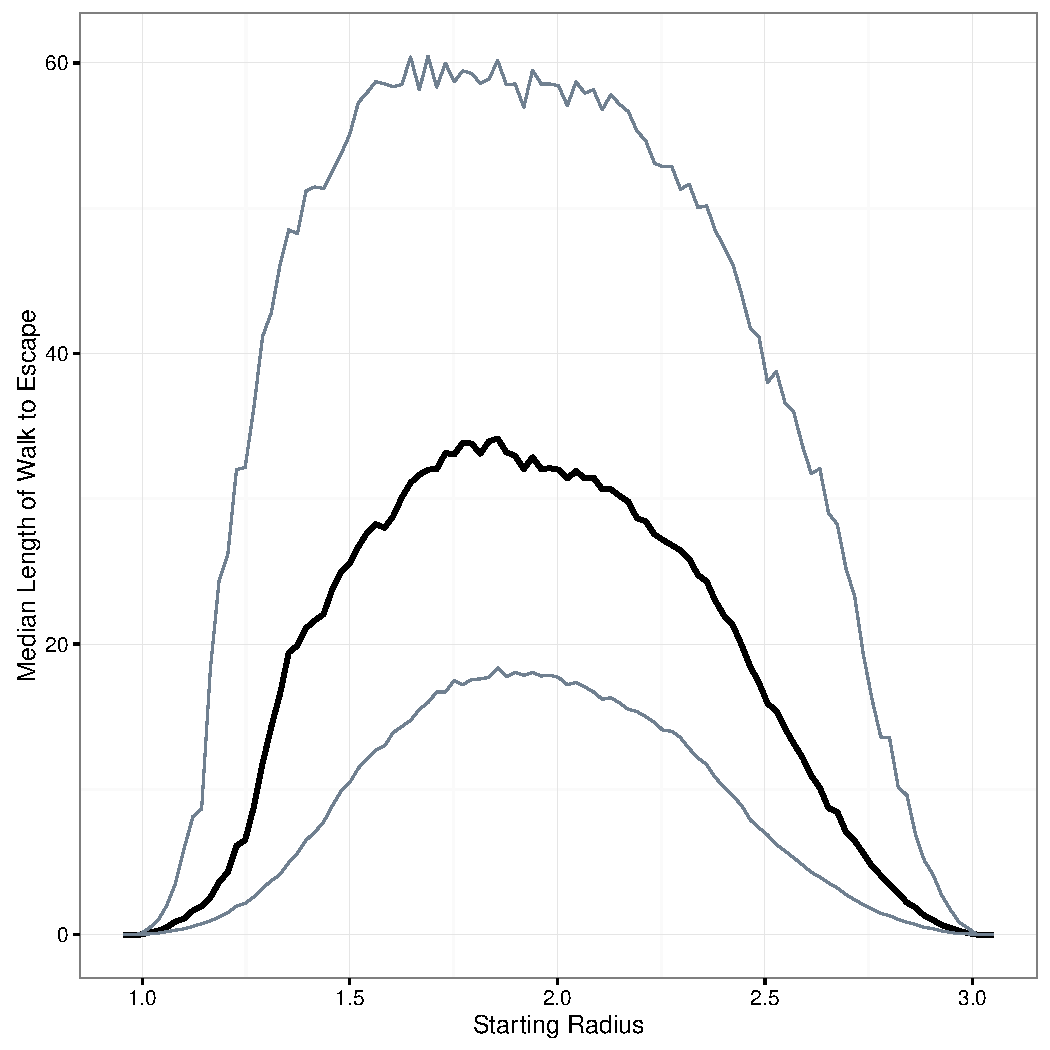
\includegraphics[width=0.85\textwidth]{images/PlaneIn1Out3.pdf}
	\end{figure}

\end{frame}

%---------------------------------------------------------------

%Circular Walls

\begin{frame}
	
	\frametitle{Plane}
	
	\begin{figure}
		% Graphic for TeX using PGF
% Title: /home/tom/CodeProjects/MathDHP_201718/RandomManifoldWalks/Presentation/images/PlaneWalls.dia
% Creator: Dia v0.97.3
% CreationDate: Mon Apr 23 12:42:27 2018
% For: tom
% \usepackage{tikz}
% The following commands are not supported in PSTricks at present
% We define them conditionally, so when they are implemented,
% this pgf file will use them.
\ifx\du\undefined
  \newlength{\du}
\fi
\setlength{\du}{15\unitlength}
\begin{tikzpicture}
\pgftransformxscale{1.000000}
\pgftransformyscale{-1.000000}
\definecolor{dialinecolor}{rgb}{0.000000, 0.000000, 0.000000}
\pgfsetstrokecolor{dialinecolor}
\definecolor{dialinecolor}{rgb}{1.000000, 1.000000, 1.000000}
\pgfsetfillcolor{dialinecolor}
\pgfsetlinewidth{0.100000\du}
\pgfsetdash{}{0pt}
\pgfsetdash{}{0pt}
\pgfsetbuttcap
\pgfsetmiterjoin
\pgfsetlinewidth{0.100000\du}
\pgfsetbuttcap
\pgfsetmiterjoin
\pgfsetdash{}{0pt}
\definecolor{dialinecolor}{rgb}{0.721569, 0.701961, 0.701961}
\pgfsetfillcolor{dialinecolor}
\pgfpathellipse{\pgfpoint{10.000000\du}{15.000000\du}}{\pgfpoint{7.500000\du}{0\du}}{\pgfpoint{0\du}{7.500000\du}}
\pgfusepath{fill}
\definecolor{dialinecolor}{rgb}{0.000000, 0.000000, 1.000000}
\pgfsetstrokecolor{dialinecolor}
\pgfpathellipse{\pgfpoint{10.000000\du}{15.000000\du}}{\pgfpoint{7.500000\du}{0\du}}{\pgfpoint{0\du}{7.500000\du}}
\pgfusepath{stroke}
\pgfsetbuttcap
\pgfsetmiterjoin
\pgfsetdash{}{0pt}
\definecolor{dialinecolor}{rgb}{0.000000, 0.000000, 1.000000}
\pgfsetstrokecolor{dialinecolor}
\pgfpathellipse{\pgfpoint{10.000000\du}{15.000000\du}}{\pgfpoint{7.500000\du}{0\du}}{\pgfpoint{0\du}{7.500000\du}}
\pgfusepath{stroke}
\pgfsetlinewidth{0.100000\du}
\pgfsetdash{}{0pt}
\pgfsetdash{}{0pt}
\pgfsetbuttcap
\pgfsetmiterjoin
\pgfsetlinewidth{0.100000\du}
\pgfsetbuttcap
\pgfsetmiterjoin
\pgfsetdash{}{0pt}
\definecolor{dialinecolor}{rgb}{1.000000, 1.000000, 1.000000}
\pgfsetfillcolor{dialinecolor}
\fill (8.032258\du,13.000000\du)--(8.032258\du,17.058333\du)--(11.959677\du,17.058333\du)--(11.959677\du,13.000000\du)--cycle;
\definecolor{dialinecolor}{rgb}{0.000000, 0.000000, 0.000000}
\pgfsetstrokecolor{dialinecolor}
\draw (8.032258\du,13.000000\du)--(8.032258\du,17.058333\du)--(11.959677\du,17.058333\du)--(11.959677\du,13.000000\du)--cycle;
\pgfsetbuttcap
\pgfsetmiterjoin
\pgfsetdash{}{0pt}
\definecolor{dialinecolor}{rgb}{0.000000, 0.000000, 0.000000}
\pgfsetstrokecolor{dialinecolor}
\draw (8.032258\du,13.000000\du)--(8.032258\du,17.058333\du)--(11.959677\du,17.058333\du)--(11.959677\du,13.000000\du)--cycle;
\pgfsetlinewidth{0.000000\du}
\pgfsetdash{}{0pt}
\pgfsetdash{}{0pt}
\pgfsetbuttcap
\pgfsetmiterjoin
\pgfsetlinewidth{0.000000\du}
\pgfsetbuttcap
\pgfsetmiterjoin
\pgfsetdash{}{0pt}
\definecolor{dialinecolor}{rgb}{0.000000, 0.000000, 0.000000}
\pgfsetfillcolor{dialinecolor}
\pgfpathellipse{\pgfpoint{10.000000\du}{15.000000\du}}{\pgfpoint{0.100000\du}{0\du}}{\pgfpoint{0\du}{0.100000\du}}
\pgfusepath{fill}
\definecolor{dialinecolor}{rgb}{0.000000, 0.000000, 0.000000}
\pgfsetstrokecolor{dialinecolor}
\pgfpathellipse{\pgfpoint{10.000000\du}{15.000000\du}}{\pgfpoint{0.100000\du}{0\du}}{\pgfpoint{0\du}{0.100000\du}}
\pgfusepath{stroke}
\pgfsetbuttcap
\pgfsetmiterjoin
\pgfsetdash{}{0pt}
\definecolor{dialinecolor}{rgb}{0.000000, 0.000000, 0.000000}
\pgfsetstrokecolor{dialinecolor}
\pgfpathellipse{\pgfpoint{10.000000\du}{15.000000\du}}{\pgfpoint{0.100000\du}{0\du}}{\pgfpoint{0\du}{0.100000\du}}
\pgfusepath{stroke}
\end{tikzpicture}

	\end{figure}
	
\end{frame}

\begin{frame}
	
	\frametitle{Plane}
	
	\begin{figure}
		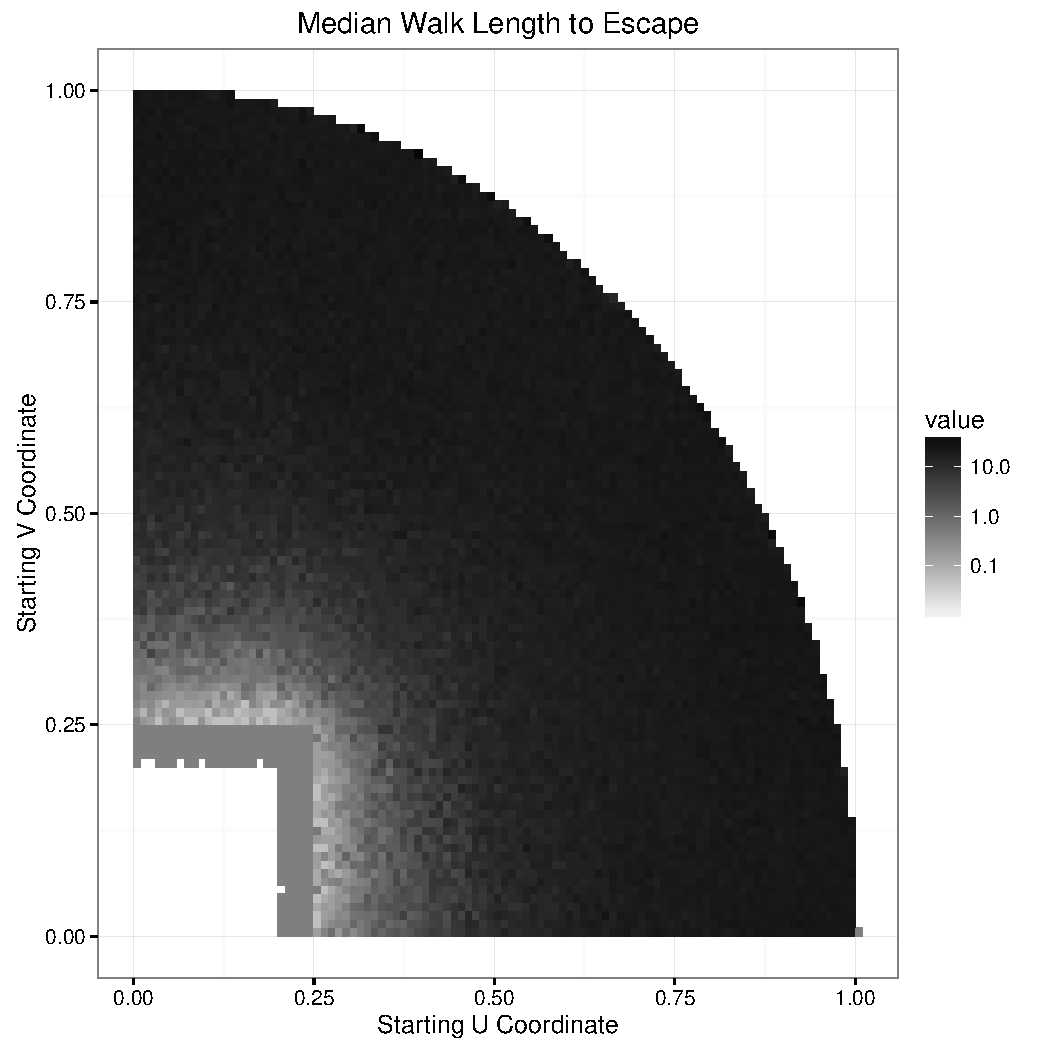
\includegraphics[width=0.85\textwidth]{images/PlaneCircleL05.pdf}
	\end{figure}
	
\end{frame}

%---------------------------------------------------------------

%Sphere Polar Escape Circle

\begin{frame}
	
	\frametitle{Sphere}
	
	\begin{figure}
		% Graphic for TeX using PGF
% Title: /home/tom/CodeProjects/MathDHP_201718/RandomManifoldWalks/Presentation/images/SpherePolar.dia
% Creator: Dia v0.97.3
% CreationDate: Mon Apr 23 12:42:31 2018
% For: tom
% \usepackage{tikz}
% The following commands are not supported in PSTricks at present
% We define them conditionally, so when they are implemented,
% this pgf file will use them.
\ifx\du\undefined
  \newlength{\du}
\fi
\setlength{\du}{12\unitlength}
\begin{tikzpicture}
\pgftransformxscale{1.000000}
\pgftransformyscale{-1.000000}
\definecolor{dialinecolor}{rgb}{0.000000, 0.000000, 0.000000}
\pgfsetstrokecolor{dialinecolor}
\definecolor{dialinecolor}{rgb}{1.000000, 1.000000, 1.000000}
\pgfsetfillcolor{dialinecolor}
\pgfsetlinewidth{0.100000\du}
\pgfsetdash{}{0pt}
\pgfsetdash{}{0pt}
\pgfsetbuttcap
\pgfsetmiterjoin
\pgfsetlinewidth{0.100000\du}
\pgfsetbuttcap
\pgfsetmiterjoin
\pgfsetdash{}{0pt}
\definecolor{dialinecolor}{rgb}{1.000000, 1.000000, 1.000000}
\pgfsetfillcolor{dialinecolor}
\pgfpathellipse{\pgfpoint{9.950000\du}{12.450000\du}}{\pgfpoint{7.450000\du}{0\du}}{\pgfpoint{0\du}{7.450000\du}}
\pgfusepath{fill}
\definecolor{dialinecolor}{rgb}{0.000000, 0.000000, 0.000000}
\pgfsetstrokecolor{dialinecolor}
\pgfpathellipse{\pgfpoint{9.950000\du}{12.450000\du}}{\pgfpoint{7.450000\du}{0\du}}{\pgfpoint{0\du}{7.450000\du}}
\pgfusepath{stroke}
\pgfsetbuttcap
\pgfsetmiterjoin
\pgfsetdash{}{0pt}
\definecolor{dialinecolor}{rgb}{0.000000, 0.000000, 0.000000}
\pgfsetstrokecolor{dialinecolor}
\pgfpathellipse{\pgfpoint{9.950000\du}{12.450000\du}}{\pgfpoint{7.450000\du}{0\du}}{\pgfpoint{0\du}{7.450000\du}}
\pgfusepath{stroke}
\pgfsetlinewidth{0.100000\du}
\pgfsetdash{}{0pt}
\pgfsetdash{}{0pt}
\pgfsetbuttcap
{
\definecolor{dialinecolor}{rgb}{0.000000, 0.000000, 0.000000}
\pgfsetfillcolor{dialinecolor}
% was here!!!
\definecolor{dialinecolor}{rgb}{0.000000, 0.000000, 0.000000}
\pgfsetstrokecolor{dialinecolor}
\draw (9.950000\du,12.450000\du)--(9.950000\du,12.450000\du);
}
\pgfsetlinewidth{0.100000\du}
\pgfsetdash{{1.000000\du}{1.000000\du}}{0\du}
\pgfsetdash{{1.000000\du}{1.000000\du}}{0\du}
\pgfsetbuttcap
{
\definecolor{dialinecolor}{rgb}{0.000000, 0.000000, 0.000000}
\pgfsetfillcolor{dialinecolor}
% was here!!!
\definecolor{dialinecolor}{rgb}{0.000000, 0.000000, 0.000000}
\pgfsetstrokecolor{dialinecolor}
\draw (9.950000\du,12.450000\du)--(9.950000\du,12.450000\du);
}
\pgfsetlinewidth{0.100000\du}
\pgfsetdash{{1.000000\du}{1.000000\du}}{0\du}
\pgfsetdash{{1.000000\du}{1.000000\du}}{0\du}
\pgfsetbuttcap
{
\definecolor{dialinecolor}{rgb}{0.000000, 0.000000, 0.000000}
\pgfsetfillcolor{dialinecolor}
% was here!!!
\definecolor{dialinecolor}{rgb}{0.000000, 0.000000, 0.000000}
\pgfsetstrokecolor{dialinecolor}
\draw (9.950000\du,12.450000\du)--(9.950000\du,12.450000\du);
}
\pgfsetlinewidth{0.100000\du}
\pgfsetdash{{1.000000\du}{1.000000\du}}{0\du}
\pgfsetdash{{1.000000\du}{1.000000\du}}{0\du}
\pgfsetbuttcap
{
\definecolor{dialinecolor}{rgb}{0.000000, 0.000000, 0.000000}
\pgfsetfillcolor{dialinecolor}
% was here!!!
\definecolor{dialinecolor}{rgb}{0.000000, 0.000000, 0.000000}
\pgfsetstrokecolor{dialinecolor}
\draw (9.950000\du,12.450000\du)--(9.950000\du,12.450000\du);
}
\pgfsetlinewidth{0.100000\du}
\pgfsetdash{{1.000000\du}{1.000000\du}}{0\du}
\pgfsetdash{{1.000000\du}{1.000000\du}}{0\du}
\pgfsetbuttcap
{
\definecolor{dialinecolor}{rgb}{0.000000, 0.000000, 0.000000}
\pgfsetfillcolor{dialinecolor}
% was here!!!
\definecolor{dialinecolor}{rgb}{0.000000, 0.000000, 0.000000}
\pgfsetstrokecolor{dialinecolor}
\draw (9.950000\du,12.450000\du)--(9.950000\du,12.450000\du);
}
\pgfsetlinewidth{0.100000\du}
\pgfsetdash{{\pgflinewidth}{0.200000\du}}{0cm}
\pgfsetdash{{\pgflinewidth}{0.200000\du}}{0cm}
\pgfsetbuttcap
{ %Axis line
\definecolor{dialinecolor}{rgb}{0.000000, 0.000000, 0.000000}
\pgfsetfillcolor{dialinecolor}
% was here!!!
\definecolor{dialinecolor}{rgb}{0.000000, 0.000000, 0.000000}
\pgfsetstrokecolor{dialinecolor}
\draw (9.900000\du,2.800000\du)--(9.950000\du,21.300000\du);
}
\pgfsetlinewidth{0.100000\du}
\pgfsetdash{}{0pt}
\pgfsetdash{}{0pt}
\pgfsetbuttcap
{ %Bottom Arc
\definecolor{dialinecolor}{rgb}{0.000000, 0.000000, 0.000000}
\pgfsetfillcolor{dialinecolor}
% was here!!!
\definecolor{dialinecolor}{rgb}{0.000000, 0.000000, 0.000000}
\pgfsetstrokecolor{dialinecolor}
\pgfpathmoveto{\pgfpoint{3.998715\du}{7.999559\du}}
\pgfpatharc{109}{72}{18.500000\du and 18.500000\du}
\pgfusepath{stroke}
}
\pgfsetlinewidth{0.050000\du}
\pgfsetdash{}{0pt}
\pgfsetdash{}{0pt}
\pgfsetbuttcap
{ %Radial vector
\definecolor{dialinecolor}{rgb}{0.000000, 0.000000, 0.000000}
\pgfsetfillcolor{dialinecolor}
% was here!!!
\pgfsetarrowsstart{stealth}
\definecolor{dialinecolor}{rgb}{0.000000, 0.000000, 0.000000}
\pgfsetstrokecolor{dialinecolor}
\draw (16.025000\du,8.056250\du)--(9.925000\du,12.050000\du);
}
\pgfsetlinewidth{0.050000\du}
\pgfsetdash{}{0pt}
\pgfsetdash{}{0pt}
\pgfsetbuttcap
{
\definecolor{dialinecolor}{rgb}{0.000000, 0.000000, 0.000000}
\pgfsetfillcolor{dialinecolor}
% was here!!!
\definecolor{dialinecolor}{rgb}{0.000000, 0.000000, 0.000000}
\pgfsetstrokecolor{dialinecolor}
\pgfpathmoveto{\pgfpoint{16.025048\du}{8.006314\du}}
\pgfpatharc{324}{217}{7.481389\du and 7.481389\du}
\pgfusepath{stroke}
}
\end{tikzpicture}

	\end{figure}
	
\end{frame}

\begin{frame}
	
	\frametitle{Sphere}
	
	\begin{figure}
		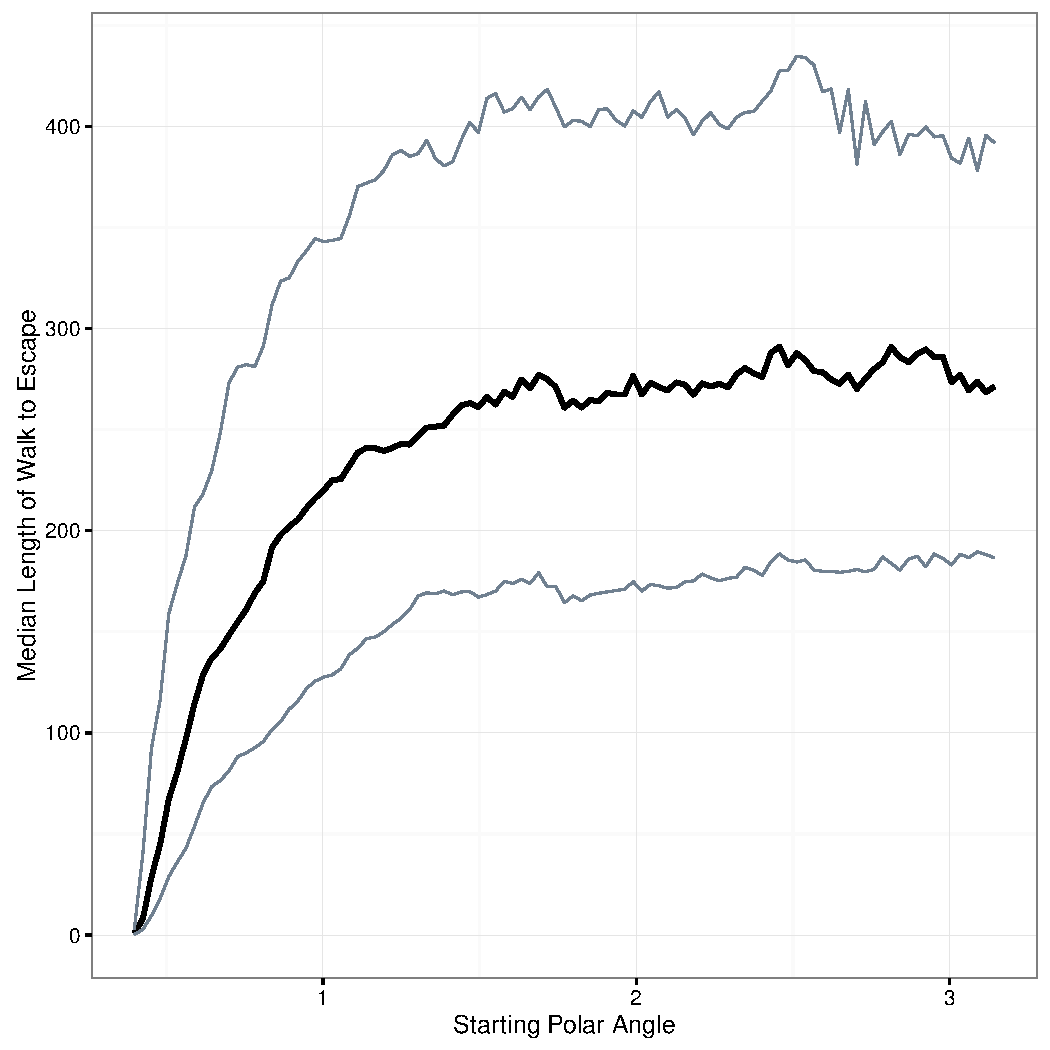
\includegraphics[width=0.85\textwidth]{images/ExampleSphereL04.pdf}
	\end{figure}
	
\end{frame}

%---------------------------------------------------------------

\begin{frame}
	
	\frametitle{Sphere}
	
	\begin{figure}
		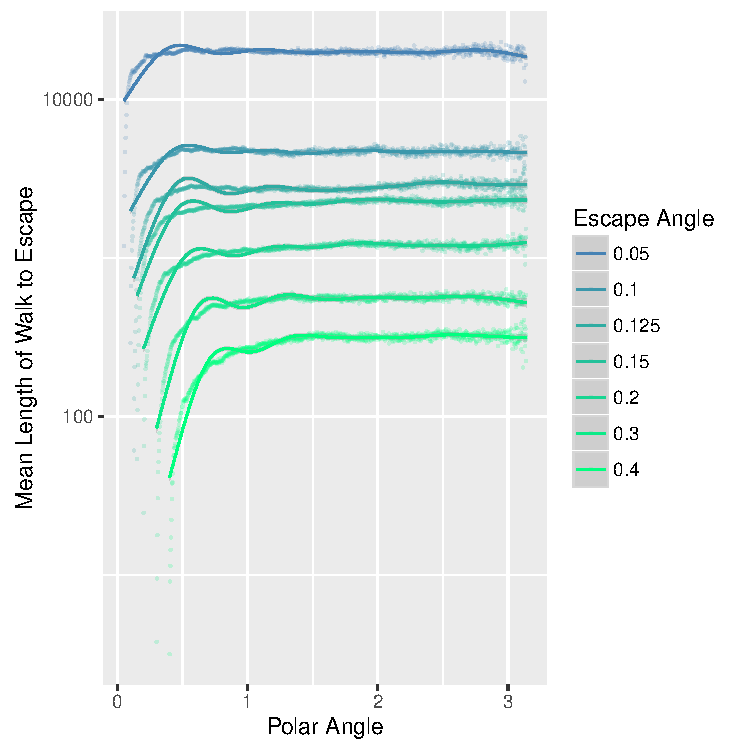
\includegraphics[width=0.85\textwidth]{images/SummaryPlot_L005_04.pdf}
	\end{figure}
	
\end{frame}

%------------------------------------------------
\section{Questions}

\begin{frame}
	
	\Huge{\centerline{Questions?}}
	
\end{frame}

\end{document} 